% !TEX root = main.tex

\documentclass[12pt, a4paper, openany]{book}
\renewcommand{\chaptername}{Capítulo}
\usepackage[utf8]{inputenc}
\usepackage{csquotes}
\usepackage[spanish]{babel}
\usepackage[
backend=biber,
style=alphabetic,
style=ieee
]{biblatex}
\addbibresource{referencias.bib}
\usepackage[skip=10pt plus1pt, indent=20pt]{parskip}
\usepackage{indentfirst}
\usepackage[acronym]{glossaries}
\usepackage{listings}
\usepackage{geometry}
\usepackage{hyperref}
\usepackage{tocbibind}
\usepackage{tikz}
\usetikzlibrary{shapes.geometric, arrows}
\tikzstyle{startstop} = [rectangle, rounded corners, minimum width=3cm, minimum height=1cm,text centered, draw=black, fill=red!30]
\tikzstyle{io} = [trapezium, trapezium left angle=70, trapezium right angle=110, minimum width=3cm, minimum height=1cm, text centered, draw=black, fill=blue!30]
\tikzstyle{process} = [rectangle, minimum width=3cm, minimum height=1cm, text centered, draw=black, fill=orange!30]
\tikzstyle{decision} = [diamond, minimum width=3cm, minimum height=1cm, text centered, draw=black, fill=green!30]
\tikzstyle{arrow} = [thick,->,>=stealth]
\geometry{left=2cm,right=2cm,top=2cm,bottom=2cm}
%
\usepackage[spanish]{babel}
\usepackage{graphicx}
\graphicspath{ {images/} }
\usepackage{placeins}
\setcounter{tocdepth}{3}
\setcounter{secnumdepth}{3}
\renewcommand\lstlistlistingname{Snippets de código}
\renewcommand{\lstlistingname}{Snippet}

%

%
\usepackage{url}
\makeglossaries
\newacronym{bof}{BOF}{Buffer Overflow}
\newacronym{usaf}{USAF}{Fuerza Aérea de los Estados Unidos}
\newacronym{x86}{i386}{Intel 386}
\newacronym{x64}{x86\_64}{AMD 64}
\newacronym{ast}{AST}{Abstract Syntax Tree}
\newacronym{yacc}{YACC}{Yet Another Compiler-Compiler}
\newacronym{libc}{LIBC}{Librería estándar C}
\newacronym{gcc}{GCC}{GNU Compiler Collection}
\newacronym{sast}{SAST}{Prueba de seguridad de aplicación estática}
\newacronym{lifo}{LIFO}{Last In, First Out}
\newacronym{bss}{BSS}{Block Starting Symbol}
\newacronym{io}{I/O}{Input/Output}
\newacronym{eax}{EAX}{Extended Accumulator Register}
\newacronym{ebx}{EBX}{Extended Base Register}
\newacronym{ecx}{ECX}{Extended Counter Register}
\newacronym{edx}{EDX}{Extended Data Register}
\newacronym{esi}{ESI}{Extended Source Index}
\newacronym{edi}{EDI}{Extended Destination Index}
\newacronym{esp}{ESP}{Extended Stack Pointer}
\newacronym{ebp}{EBP}{Extended Base Pointer}
\newacronym{eip}{EIP}{Extended Instruction Pointer}
\newacronym{gdb}{GDB}{GNU Debugger}
\newacronym{nx}{NX}{No eXecute}
\newacronym{nop}{NOP}{No Operation}
\newacronym{ret}{RET}{Return}
\newacronym{aslr}{ASLR}{Address Space Layout Randomization}
\newacronym{pie}{PIE}{Position Independant Executable}
\usepackage{xcolor}

\definecolor{codegreen}{rgb}{0,0.6,0}
\definecolor{codegray}{rgb}{0.5,0.5,0.5}
\definecolor{codepurple}{rgb}{0.58,0,0.82}
\definecolor{backcolour}{rgb}{0.95,0.95,0.92}

\lstdefinestyle{mystyle}{
    backgroundcolor=\color{backcolour},   
    commentstyle=\color{codegreen},
    keywordstyle=\color{magenta},
    numberstyle=\tiny\color{codegray},
    stringstyle=\color{codepurple},
    basicstyle=\ttfamily\footnotesize,
    breakatwhitespace=false,         
    breaklines=true,                 
    captionpos=b,                    
    keepspaces=true,                 
    numbers=left,                    
    numbersep=5pt,                  
    showspaces=false,                
    showstringspaces=false,
    showtabs=false,                  
    tabsize=2
}

\lstset{style=mystyle}
\begin{document}
\chapter*{Abstract}
\section*{Resumen}
En este proyecto se ha desarrollado un sistema capaz de generar desafíos de ciberseguridad en la categoría de explotación binaria a partir de códigos en lenguaje C legítimos.
El sistema toma estos códigos y, mediante un procesamiento avanzado, introduce vulnerabilidades que permiten la creación de escenarios de aprendizaje.
El programa facilita la práctica de técnicas de explotación binaria al convertir código seguro en retos que simulan fallos de seguridad reales.
Además, se han implementado soluciones explicativas que ayudan a los usuarios del programa a comprender el proceso de explotación y mejorar sus habilidades en ciberseguridad.
Esta herramienta es útil tanto para principiantes como para expertos que deseen perfeccionar sus conocimientos en la identificación y explotación de vulnerabilidades.

\section*{Palabras clave}
Ciberseguridad, Explotación de binarios, Static Application Security Testing, SAST, Abstract Syntax Tree, AST, Código C, Assembly, PWN, Python, GDB
\printglossary[type=\acronymtype]
\tableofcontents
\chapter[Introducción]{Introducción}
% \section*{Introducción}
Con el paso del tiempo, la ciberseguridad se ha convertido en un campo de mucha relevancia
en el sector de las telecomunicaciones e informática.

Desde la invención y adopción de internet, los equipos informáticos cada día están más expuestos
al mundo, y debido a esto, es de vital importancia asegurarse que estos dispositivos son seguros y no tienen vulnerabilidades que puedan permitir a un actor maligno tomar el control.

La vulnerabilidad del tipo `\acrfull{bof}' o `Desbordamiento de buffer', fue una de las primeras vulnerabilidades usadas para explotar sistemas remotos sin interacción de los usuarios. El mecanismo de explotación fue documentado por primera vez en 1972 por la \acrfull{usaf}, sin embargo, no fue hasta 1988 cuando se descubrió el primer gusano llamado Morris \cite{Morris} el cual entre las diferentes técnicas de explotación hacía uso de un \acrshort{bof} sobre el servicio `fingerd' \cite{Fingerd}.

Con el paso del tiempo y debido a los nuevos lenguajes de programación que han ido surgiendo, los \acrshort{bof} se han vuelto menos comunes, debido a que estos nuevos lenguajes abstraen al usuario de la gestión de la memoria e interactúan con el sistema de una forma más segura y controlada. Sin embargo, esta vulnerabilidad sigue siendo crítica, ya que aunque el lenguaje abstraiga al programador de la gestión de memoria, el propio compilador del lenguaje podría tener este tipo de errores o alguna librería externa que se inserte en el código.

Este trabajo fin de estudios se centra en el desarrollo de un sistema automatizado para la generación de códigos en lenguaje C que contienen vulnerabilidades intencionales. Este sistema permite a los usuarios practicar diversas técnicas de explotación de binarios, como el \acrshort{bof}, la ejecución de código arbitrario y la manipulación de la memoria, en un entorno seguro y educativo. Al proporcionar códigos vulnerables de manera automatizada, el proyecto busca facilitar el proceso de aprendizaje, permitiendo a los estudiantes enfocarse en la identificación y explotación de vulnerabilidades en lugar de en la creación de escenarios manualmente.

\chapter[Estado del arte]{Estado del arte}
% \section*{Estado del arte}
En el análisis del estado del arte de las herramientas de ciberseguridad, se identifican diversas aplicaciones que permiten analizar y explotar binarios de forma automática.
Entre las más relevantes se encuentran `pwntools' la cual es un framework de explotación que permite automatizar muchas funcionalidades y tiene una función de autoexplotación de binarios mediante `Corefiles'.
Otra herramienta es `rex' del equipo de `angr', sin embargo no es sencilla de instalar además de que carece de estabilidad en su ejecución.
Estas herramientas son eficaces para la identificación de vulnerabilidades y la explotación automatizada, pero se enfocan principalmente en la evaluación de binarios existentes y no en la creación de desafíos personalizados para la enseñanza.

Sin embargo, no se han encontrado programas que ofrezcan la generación automática de retos de explotación binaria a partir de códigos C legítimos.
Esta carencia subraya una oportunidad significativa en el campo de la ciberseguridad educativa, donde hay una necesidad creciente de recursos didácticos que permitan a los estudiantes practicar de manera segura con escenarios realistas.
El desarrollo de una herramienta que automatice la generación de estos retos no solo podría revolucionar la enseñanza de la explotación de binarios, sino que también facilitaría un aprendizaje práctico, permitiendo a los estudiantes enfrentarse a una variedad de vulnerabilidades en un entorno seguro y controlado.

Este proyecto responde a esa necesidad al proporcionar un sistema que convierte códigos C seguros en desafíos de explotación.
Al hacerlo, se ofrece una solución innovadora que fomenta un enfoque más práctico y orientado a la formación en materia de ciberseguridad, brindándoles la experiencia y habilidades necesarias para identificar y mitigar vulnerabilidades en binarios.
\chapter[Desarrollo técnico]{Desarrollo técnico}
En esta sección se describe técnicamente parte por parte cómo se ha planificado el proyecto. El trabajo está dividido en tres secciones: análisis del código C, inyección de vulnerabilidades y soluciones a los retos.

En la primera sección, se explican las herramientas utilizadas para analizar los códigos fuentes de entrada y como se manejan los mismos.

La segunda sección, explica los diferentes tipos de vulnerabilidades que se pueden inyectar y como se modifica el código fuente original para poder incluir estos nuevos flujos y funciones vulnerables.

En la tercera y última sección, se explican los diferentes mecanismos de resolución del problema y cómo son entregados al usuario.
\section{Análisis del código fuente}
El proyecto está desarrollado en `Python', un lenguaje de programación sencillo que permite de forma rápida crear prototipos. En esta sección se describen las librerías, lógica y flujos que utiliza el programa.

\subsection{Preparación del entorno}
El desarrollo se ha realizado en un sistema operativo del tipo Linux, en concreto sobre la distribución de `Fedora', el software de este proyecto es compatible con cualquier sistema operativo de la familia Linux, que opere sobre arquitecturas del tipo \acrfull{x86} o \acrfull{x64}.

Más adelante se explican las diferencias que tienen en la traducción al código máquina. Este programa va a trabajar mayoritariamente con la arquitectura \acrshort{x86}.

Las dependencias del sistema necesarias para trabajar con el proyecto son las siguientes:
\begin{itemize}
    \item Sistema operativo
    \begin{itemize}
        \item \acrshort{gcc}
        \item glibc-devel.i686 (Paquete para compilar binarios de 32bit)
        \item glibc-devel.x86\_64
        \item python3.12
        \item poetry \cite{poetry-install}
        \item gdb
        \item gdb-server
        \item make
        \item objdump
    \end{itemize}
    \item Librerías de Python para el proyecto
    \begin{itemize}
        \item pycparser \cite{pycparser}
        \item pwntools \cite{pwntools}
        \item structlog \cite{structlog}
    \end{itemize}
\end{itemize}

Las librerías de Python, se pueden instalar de forma automática mediante el gestor de paquetes `Poetry', para ello dentro del repositorio del proyecto, nos colocaremos en la carpeta `src' y podemos ejecutar dos comandos diferentes para conseguir el mismo objetivo, cualquiera de los dos instalará las dependencias necesarias a nivel de Python.

\begin{lstlisting}[language=bash]
# Usando el fichero Makefile
make init

# Comando manual de Poetry
poetry install
\end{lstlisting}

\subsection{Explicación del sistema AST}
El proyecto, hace uso de los \acrfull{ast} \cite{ast}. Un \acrshort{ast}, es una estructura de datos en forma de árbol que representa la estructura sintáctica abstracta de un texto escrito en un lenguaje formal, como código fuente. Cada nodo del árbol representa una construcción que ocurre en el texto. Los \acrshort{ast} son usados ampliamente en compiladores porque representan la estructura del código de un programa. La sintaxis abstracta se caracteriza por no incluir todos los detalles que se encuentran en la sintaxis concreta. Por ejemplo, la estructura de árbol subyacente implica el agrupamiento de los paréntesis, y una construcción sintáctica como IF condición THEN puede representarse con un único nodo que tenga dos ramas.

Esto es un ejemplo donde conviete el siguiente código Python sobre el algoritmo euclidiano a un \acrshort{ast}, mostrado en la figura \ref{fig:ast}:

\begin{lstlisting}[language=Python, caption=Python - Algoritmo euclidiano]
def euclidean(a: int, b: int) -> int:
    while b != 0:
      if a > b:
        a -= b
      else:
        b -= a
    return a
\end{lstlisting}

\begin{figure}[htb!]
      \centering                        
      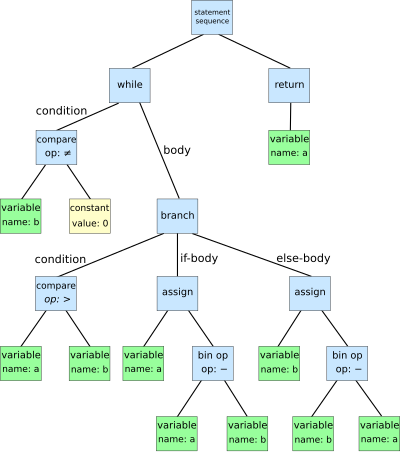
\includegraphics[width=0.8\textwidth]{images/AST.png}
      \caption{Algoritmo euclídeo en formato \acrshort{ast} }
      \label{fig:ast}
\end{figure}
\FloatBarrier
Como se puede observar en la figura \ref{fig:ast} este formato de árbol - rama no es sencillo de interpretar para un humano, sin embargo, de forma programática se puede analizar y/o alterar la estructura de forma relativamente sencilla.

El funcionamiento de la librería es complejo, por debajo emplea el metodo Lex (Lexer) - \acrfull{yacc}. Está implementado usando la librería `PLY' \cite{ply}, la cual es una herramienta que tokeniza el código y mediante funciones que analizan estos tokens permite construir un \acrshort{ast}, que es lo que realiza la herramienta `pycparser'.

\subsection{Análisis del código C con Python}
El software desarrollado implementa dos clases principales. La primera clase se encarga de procesar el código C, convertirlo en un \acrshort{ast} utilizando la librería `pycparser', y modificar este árbol para introducir cambios estructurales, como por ejemplo, las vulnerabilidades, esta clase se llama `AstProcessor'. La segunda clase se especializa en analizar el \acrshort{ast} generado, buscando puntos críticos donde se puedan inyectar vulnerabilidades de manera deliberada, tiene el nombre de `VulnGen'.

\subsubsection{AstProcessor} \label{subsub:astproc}
Esta clase de Python únicamente hace uso de la librería `pycparser'. En ella se han implementado todas las funcionalidades importantes que permiten analizar, modificar, guardar y compilar el código.

El flujo para el procesado del código fuente comienza mediante el cargado del fichero en la librería. Para traducir el archivo a un \acrshort{ast}, el paquete hace uso de unas cabeceras modificadas de la \acrfull{libc} y del compilador \acrfull{gcc}. Para ello, las flags que se han añadido en el compilador son las siguientes:
\begin{itemize}
    \item -E : Afecta al enlazamiento de librerías
    \item -nostdinc : No incluir las librerías por defecto del sistema, por ejemplo, `string.h'
    \item -Iutils/fake\_libc\_include : Incluir las cabeceras falsas de libc para que el compilador no arroje errores
\end{itemize}

Una vez procesado el código al formato \acrshort{ast}, se hace un preprocesado de las secciones de interés para facilitar posteriores modificaciones y búsquedas de objetos. La clase dispone de 8 objetos principales diferentes:
\begin{itemize}
    \item ast: aquí se almacena todo el procesado obtenido por `pycparser'.
    \item astjson: lo mismo que en el objeto `ast', sin embargo, está en formato diccionario
    \item typedefs:  son definiciones de variables y tamaños sobre el nucleo de C.
    \item code: la subestructura del \acrshort{ast} con el código fuente importante, sin definiciones de tipos.
    \item funcs: diccionario con las definiciones de funciones
    \item globals: diccionario con variables globales o declaradas fuera de la función `main'
    \item vars: diccionario con todas las variables divididas en globales y funciones
    \item fncalls: diccionario con todas las llamadas a funciones divididas por función origen
\end{itemize}

Aprovechando el funcionamiento de las clases en Python, una modificación en cualquiera de los objetos enlazados entre variables repercutirá directamente sobre el objeto original debido a que el lenguaje referencia el valor original en vez de generar una nueva copia.

Para trabajar con el \acrshort{ast}, es muy importante entender el funcionamiento de los `scope' cuando se usa una variable en el código. El compilador primero intenta ubicar la variable en la función donde se está ejecutando, y en caso de no encontrar la variable, probará a buscarla de nuevo en el entorno global, siendo estrictos con la definición, un scope se define como código aislado entre dos llaves `\{\}'. Esto se puede comprobar con el siguiente código:
\pagebreak
\begin{lstlisting}[language=C, caption=Scopes en C]
int a = 1;
void b(){
    int a = 2;
    {
        int a = 3;
        printf("Subscope en la funcion b: %d\n", a);
    }
    printf("En la funcion b: %d\n", a);
}
int main()
{
    printf("En la funcion main: %d\n", a);
    b();
    return 0;
}
\end{lstlisting}

En el resultado se puede ver que arroja un texto con valor numérico diferente según el scope donde fue ejecutada la instrucción de imprimir por pantalla.

\subsubsection{\acrshort{sast}} \label{subsub:sast}
\acrshort{sast} es la clase encargada de localizar posibles funciones peligrosas.
Se hace uso de los \acrshort{ast} y se analiza de forma recursiva el árbol tratando de simular un procesado del `stack'. El concepto de `stack' se explica en el apartado \ref{subsub:bofstack}.

A día de la entrega del proyecto, la funcionalidad es reducida debido a que no es capaz de localizar vulnerabilidades. Cuando se procesan los diferentes tipos de asignaciones y llamadas, se revisa cuales de estas pueden ser peligrosas basado en una lista de llamadas a funciones que tratan con buffers o entrada del usuario.
Cuando se detecta una llamada peligrosa, por ejemplo, un `scanf', se genera un `problema' con todos los datos relevantes sobre la llamada: scope, stack (representa bajo qué condición se llama la función) y el \acrshort{ast} de la llamada.

Según las condiciones en las cuales se ha ejecutado la función vulnerable, se da un veredicto sobre si es un punto de inyección de vulnerabilidades, por ejemplo:

\begin{lstlisting}[language=C, caption=Funciones peligrosas]
int a = 1;
char buffer[128];
// Este codigo es una funcion vulnereable
scanf("%s %d", buffer, &a);

// Este codigo es una funcion no vulnerable
scanf("%d %d", buffer, &a);
\end{lstlisting}

\subsubsection{VulnGen}
Esta clase de Python es la encargada de realizar un análisis del \acrshort{ast} e inyectar las vulnerabilidades propuestas en la sección \ref{subsec:vulns}. Es la clase más compleja del software debido a que tiene que ser capaz de encontrar funciones que permitan sustituirlas por sus análogas vulnerables, asegurando que la explotación sucede en el punto esperado.

La clase se construye sobre otras dos clases importantes: AstProcessor explicada en el punto \ref{subsub:astproc} y la clase SAST mostrada anteriormente \ref{subsub:sast}, encargada de revisar el código y localizar posibles funciones peligrosas.

El flujo de trabajo es el siguiente:

\begin{enumerate}
    \item Se inicializa la clase VulnGen
    \begin{enumerate}
        \item Se inicializa la clase \acrshort{sast}
        \item Se procesa todo el código \acrshort{ast}
    \end{enumerate}
    \item Se analizan los problemas recogidos en \acrshort{sast}
    \begin{enumerate}
        \item Se revisa si es intercambiable de forma directa, afecta a funciones con inputs del tipo `scanf' por ejemplo
        \item En caso de no ser intercambiable, se analiza que argumento pudiera ser vulnerable y se divide la función en componentes
        \item El problema original se aisla con el componente vulnerable
    \end{enumerate}
    \item Se crea la vulnerabilidad relacionada con un nivel de dificultad
    \item Se cambia el tamaño del buffer vulnerable de forma aleatoria
    \item Se fija el buffer donde se devuelven los datos al mismo tamaño que el original
    \item Se intercambia la función original por la vulnerable, asegurando la misma funcionalidad
\end{enumerate}

Este flujo se representa gráficamente a continuación:


\begin{tikzpicture}[node distance=2cm]
        \node (start) [startstop] {VulnGen};
        \node (sast) [process, right of=start, xshift=1.5cm] {Iniciar \acrshort{sast}};
        \node (stack) [process, right of=sast, xshift=1.5cm] {Crear stack};
        \node (problemas) [process, right of=stack, xshift=2cm] {Procesar problemas};
        \node (intercambiable) [decision, below of=problemas, yshift=-1cm] {¿Intercambiable?};
        \node (fmtstr) [process, left of=intercambiable, xshift=-2.5cm] {Dividir función};
        \node (aislar) [process, left of=fmtstr, xshift=-2cm] {Aislar problema};
        \node (genvuln) [process, below of=aislar, yshift=-0.5cm] {Generar vulnerabilidad};
        \node (bufvuln) [process, below of=genvuln] {Aleatorizar buffer vulnerable};
        \node (buforig) [process, below of=bufvuln, xshift=-1.25cm] {Fijar buffer original en fn vulnerable};
        \node (intercambiofn) [process, right of=buforig, xshift=4.5cm] {Intercambio de funciones};
        \node (fin) [startstop, right of=intercambiofn, xshift=2.5cm] {Fin};
        \draw [arrow] (start) -- (sast);
        \draw [arrow] (sast) -- (stack);
        \draw [arrow] (stack) -- (problemas);
        \draw [arrow] (problemas) -- (intercambiable);
        \draw [arrow] (intercambiable) -- node[anchor=south] {no} (fmtstr);
        \draw [arrow] (intercambiable) |- node[anchor=west] {si} (genvuln);
        \draw [arrow] (fmtstr) -- (aislar);
        \draw [arrow] (aislar) -- (genvuln);
        \draw [arrow] (genvuln) -- (bufvuln);
        \draw [arrow] (bufvuln) -- (buforig);
        \draw [arrow] (buforig) -- (intercambiofn);
        \draw [arrow] (intercambiofn) -- (fin);
\end{tikzpicture}

A modo de ejemplo, el proceso puede resumirse en una entrada y una salida, tal y como se muestra en el siguiente bloque de código.
\pagebreak
\begin{lstlisting}[language=C, caption=Entrada y salida de VulnGen]
// Codigo de entrada
void main(){
 char buffer[32];
 int buffer2;
 printf("dame tu nombre y tu edad separado por espacios: ");
 scanf("%s %d",buffer,&buffer2);
 printf("Tu nombre es %s y tu edad es %d\n", buffer, buffer2);
}

// Codigo de salida
void input_66(char *buf){
  char filler[837];
  char buffer[32];
  scanf("%s", buffer);
  strcpy(buf, buffer);
}

void main(){
  char buffer[32];
  int buffer2;
  printf("dame tu nombre y tu edad separado por espacios: ");
  input_66(buffer);
  scanf(" %d", &buffer2);
  printf("Tu nombre es %s y tu edad es %d\n", buffer, buffer2);
}
\end{lstlisting}

Como se puede observar en el ejemplo, la función vulnerable `scanf' se ha dividido en dos llamadas.
La llamada para introducir el nombre en el buffer se intercambia por una función con el formato `input\_XXX' que toma como argumento el buffer destino.
Además se añade una segunda llamada a la función `scanf' únicamente para procesar el entero manteniendo el comportamiento original.

\section{Vulnerabilidades}
Esta sección se centra en explicar qué es un \acrfull{bof}, cómo ocurre, y por qué es tan peligroso.
Además, se explorán las diferentes técnicas de explotación y las mitigaciones introducidas en el paso del tiempo para reducir el riesgo de ataques críticos.
Comprender los fundamentos y las implicaciones de los desbordamientos de buffer es esencial dado que sigue siendo una amenaza vigente en muchos sistemas actuales.
\subsection{Buffer Overflow}
Un \acrfull{bof} o desbordamiento de buffer sucede cuando el tamaño del buffer donde se almacenan los datos es menor a la cantidad insertada.
En la siguiente figura se puede ver en un ejemplo gráfico.
\begin{figure}[htb!]
    \centering                        
    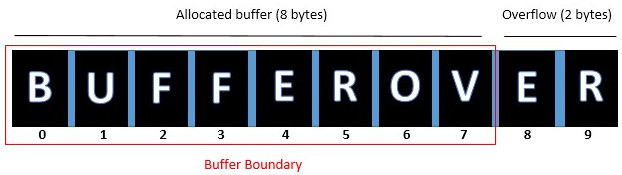
\includegraphics[width=0.8\textwidth]{images/BOF-Example.jpg}
    \caption{Ejemplo de un \acrlong{bof} }
    \label{fig:bofexample}
\end{figure}
\FloatBarrier
En el caso arriba descrito la variable que contiene el texto tiene un tamaño de 8 bytes, sin embargo, se han introducido 10 suponiendo un overflow de 2 bytes.

\subsubsection{Arquitectura de memoria Intel de 32bits}
Para la redacción de este apartado ha sido muy relevante la información contenida en el libro `Assembly Language for x86 Processors' \cite{x86asm} debido a que se explica de forma detallada el funcionamiento interno de los ejecutables en lenguaje máquina.

La arquitectura del tipo x86 se basa en una construcción del tipo `stack'. Un stack en el ámbito informático representa una estructura de datos que sigue el principio `\acrfull{lifo}', es decir, el último dato en entrar al stack es el primero en salir. Una operación del tipo `push' añadirá un dato al final del stack y la operación del tipo `pop' lo retirará.

La memoria del programa se divide en segmentos dependiendo de los datos a contener, en la siguiente lista se muestra en orden la estructura de memoria del programa:
\begin{itemize}
    \item Stack: Contiene la pila de llamadas y algunas variables. Crece en dirección del heap.
    \item Heap: Memoría reservada de forma dinámica. Crece en dirección del stack.
    \item \acrfull{bss}: Variables estáticas no inicializadas.
    \item Datos (Data): Contiene variables estáticas inicializadas, tanto locales como globales.
    \item Código (Text): Se almacenan las instrucciones a ejecutar, solo lectura-ejecución.
\end{itemize}

Para entender correctamente la convención de llamadas en esta arquitectura es importante conocer los diferentes registros y su contenido que se muestran a continuación:
\begin{itemize}
    \item \acrfull{eax}: Registro usado en operaciones aritméticas.
    \item \acrfull{ebx}: Apunta a la base del segmento de datos.
    \item \acrfull{ecx}: Contador usado normalmente en bucles.
    \item \acrfull{edx}: Puntero a operaciones de \acrshort{io}, también usado en operaciones aritméticas.
    \item \acrfull{esi}: Puntero a datos en el segmento `data', usado con strings o I/O.
    \item \acrfull{edi}: Puntero a datos o destino en el segmento `data', usado con strings o \acrshort{io}.
    \item \acrfull{esp}: Apunta a la parte superior del stack.
    \item \acrfull{ebp}: Apunta a la base del stack.
    \item \acrfull{eip}: Apunta a la siguiente instrucción a ejecutar.
\end{itemize}

La sección del stack está dividida en ventanas con los contextos de ejecución de cada función. Es decir, cada vez que se llame a una función se crea un nuevo `stack frame' con la estructura que se muestra en las siguientes figuras.

\begin{figure}[htb!]
    \centering                        
    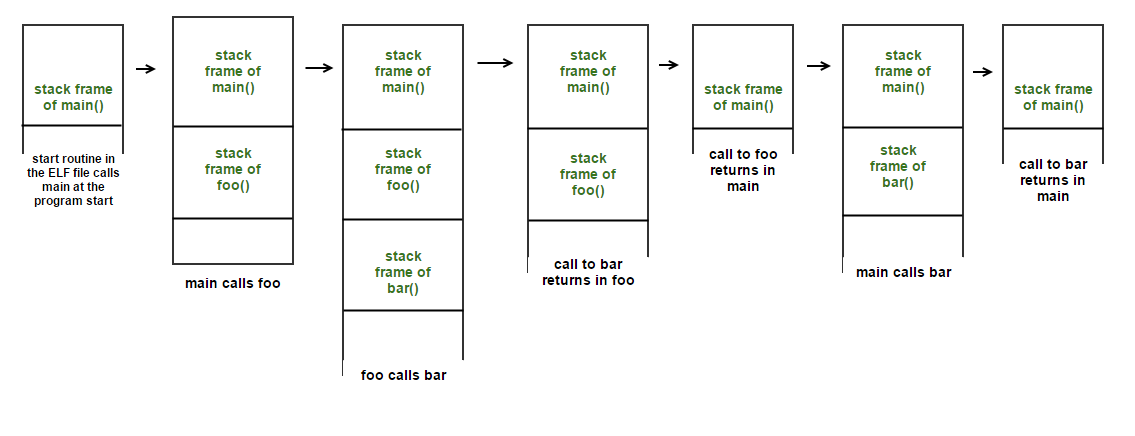
\includegraphics[width=0.8\textwidth]{images/stack-funcs.png}
    \caption{Ejemplo de crecimiento del stack}
    \label{fig:stack-funcs}
\end{figure}
\FloatBarrier
\begin{figure}[htb!]
    \centering                        
    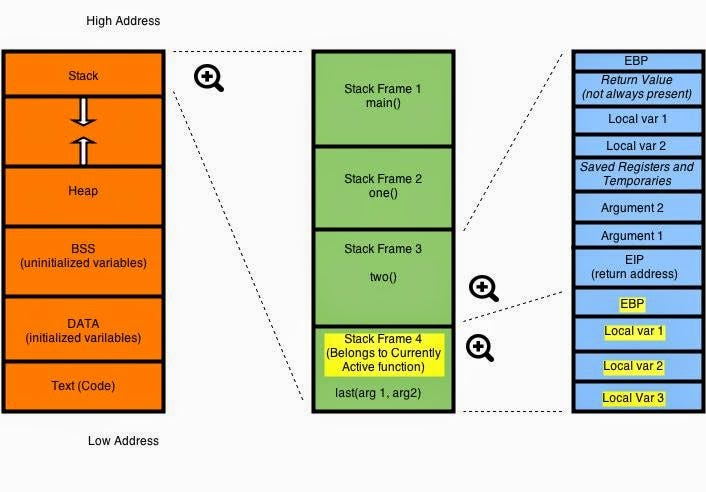
\includegraphics[width=0.8\textwidth]{images/stack-arch.jpg}
    \caption{Ejemplo a bajo nivel del contenido del stack }
    \label{fig:stack-arch}
\end{figure}
\FloatBarrier
\subsubsection{Explotando un buffer overflow en 32bits}
Con el conocimiento adquirido en el punto anterior se puede observar que si se modifica el valor del \acrshort{eip}, el programa verá alterado su flujo normal de trabajo. En este caso, en ese registro se puede establecer una dirección de memoria maligna que permita ejecutar código arbitrario.

En el siguiente código C de ejemplo se puede observar que tenemos declarada una función peligrosa llamada `ret2win'. Esta no se ejecuta en ningún momento en el código, sin embargo, existe y puede ser ejecutada alterando el flujo normal del programa.

\begin{lstlisting}[language=C, caption=Código vulnerable con función ret2win]

void ret2win(){
    system("/bin/sh");
}

void funcion_vulnerable(){
    char buffer[128];
    printf("Dime algo: ");
    gets(buffer);
    printf("\nHas escrito: %s", buffer);
}

void main(){
    printf("Esto es un programa de prueba\n");
    funcion_vulnerable();
    printf("Adios!");
}
\end{lstlisting}
\FloatBarrier
En este caso, la función `gets' permite escribir por encima del tamaño del buffer y alterar el stack pudiendo cambiar el valor del \acrshort{eip} guardado.

Es probable que compilando el código tal y como está el compilador nos arroje varias alertas sobre el fallo, además los compiladores en la actualidad implementan mitigaciones por defecto para evitar situaciones no deseadas.
Estas mitigaciones se explican en el punto \ref{subsec:mitigaciones}.
Para probar el la explotación antes descrita necesitamos compilar el binario con el siguiente comando:
\begin{lstlisting}[language=bash, caption=Compilado de código con pocas mitigaciones y arquitectura 32bit]
gcc -m32 -no-pie -fno-stack-protector -o ret2win.o ret2win.c
\end{lstlisting}

\subsection{Mitigaciones introducidas en el compilado} \label{subsec:mitigaciones}
\subsection{Evasión de mitigaciones}
\subsection{Inyección de vulnerabilidades} \label{subsec:vulns}
\section{Soluciones a los retos}
\subsection{Tutoriales}
\subsection{Ejemplos de payloads}
\chapter[Conclusiones]{Conclusiones}
En este proyecto se ha desarrollado un programa que permite la introducción de código en lenguaje C como entrada, y si se cumplen ciertas condiciones, devuelve el código fuente, el binario compilado y un `script' de ayuda que explica el proceso de resolución.
El software se estructura en tres componentes principales: el procesamiento de código C, la inyección de vulnerabilidades y la generación del método de resolución.

Durante el procesamiento del código, se ha demostrado que trabajar con un formato \acrfull{ast} facilita significativamente la gestión de las llamadas a funciones y permite la inyección nativa de definiciones de funciones, llamadas a funciones y código arbitrario en Python. Este enfoque ha simplificado el manejo del código fuente y ha mejorado la flexibilidad del software para diferentes aplicaciones.

La inyección de vulnerabilidades, por otro lado, ha presentado desafíos notables debido a la variabilidad introducida por las optimizaciones del compilador, lo que puede llevar a comportamientos inesperados. Aunque el programa permite controlar la salida del código C, no garantiza un comportamiento idéntico tras compilaciones sucesivas, especialmente en vulnerabilidades del tipo ‘format string’. Esta variabilidad ha sido un obstáculo significativo al intentar generar tutoriales consistentes para la resolución de problemas, ya que la ubicación de los offsets puede cambiar entre compilaciones, dificultando la predicción y aprendizaje.

A pesar de estas limitaciones, el software en su estado actual es una herramienta valiosa para usuarios con conocimientos básicos en la explotación de binarios. Les permite practicar y aprender sobre la explotación de ejecutables con fallas, incluso cuando todas las protecciones están activadas.
El funcionamiento del programa ha sido verificado con varios códigos fuente, incluidos en la carpeta ‘examples’ del repositorio, que pueden ser utilizados por los usuarios como punto de partida para experimentar.
% \chapter[Continuidad del proyecto]{Continuidad del proyecto}
% TODO
\printbibliography[
heading=bibintoc,
title={Referencias}
]
\listoffigures
\lstlistoflistings
\end{document}